\chapter{Introduction}
\def\thisDir{ch01-intro}
\tikzsetfigurename{ch01fig}
\glsresetall
\myEpigraph{It's a dangerous business, Frodo, going out your door. You step onto the road, and if you don't keep your feet, there's no knowing where you might be swept off to.}{John Ronald Reuel Tolkien}{The Fellowship of the Ring}

\section{Modeling}
Models play an important role in today's world, even though we often are not always aware of them.
In particular, models enable us to predict the future (within a certain bound of uncertainty):
\begin{itemize}
  \item supermarkets try to predict how many produce their patrons will buy such that they can order a large enough supply,
  \item traders on the stock market aim to predict whether companies such as Tesla or Apple will continue to prosper over the next quarter such that they can decide if it's time to buy more stock or rather sell,
  \item weather forecasters hope to predict what weather it might become tomorrow,
  \item how much electricity will the whole country use next week (do we need to start up a new power plant or not),
\end{itemize}
and so on.

Models help us to keep an oversight of complicated matters.
Once we understand the behavior of a few systems, this offers great opportunities to understand how those systems work together or even how we can control the world around us.
For engineers, models enable us to design larger and more complicated things than ever before.
E.g. consider a \gls{CPU} in a computer: with a few billion transistors, it is no longer possible for a sole human being to understand what every single transistor does in the grand scheme.
Instead, models of larger parts of the circuit allow us to retain insight (`this part of the \gls{CPU} caches some variables', `these transistors multiply two numbers', and so on).

\subsection{How to Obtain a Model?}

To successfully model a system, one has to delimit what part of the world one actually wants to model, i.e. the \term{system}.
Since a system is mostly useful if it interacts with the world around it, one often also has to define \term{inputs} through which one can influence the system, and \term{outputs} which are influenced by the system.


Modeling can be divided into two diametrical groups depending on what one uses as a starting point.
\paragraph{White box}
One the one hand, there is so-called \term{`white box'} modeling, or first-principles modeling.
The model is constructed by writing down the equations that govern the system, e.g. Newton's laws of motion for mechanical systems, Kirchoff's laws for electrical circuits, \latin{etc.}
This is the typical kind of modeling practiced in school.
Unfortunately, white box modeling quickly becomes unwieldy once more complicated systems are to be studied or many parts of the system are uncertain.
In general, lot of man-hours are required to build a white box model, such that this is often prohibitively expensive for engineering applications.

\paragraph{Black box}
On the other hand, the diametrically opposed approach is called \term{`black box'} modeling.
Here, the model structure is chosen such that a wide variety of phenomena can be described.
Regardless of the nature of the underlying system, be it mechanical, chemical, electrical, structural, \ldots; most dynamic phenomena can be described using differential equations (or difference equations).
In particular, for black-box models, the structure of the model is chosen such that the data is well-approximated.
The downside of this is that interpreting the model physically is not always possible.
Fortunately, the goal of a model is often not to interpret the physical reality but to approximate it well enough to allow engineering

\paragraph{Gray box}
Obviously, in practice nothing is ever as black and white, and neither is modeling.
In many cases, one can or even has to incorporate knowledge about the physics of the system in the modeling process.
In particular when one has black box models where some parameters are related to physical phenomena, the resulting model is called \term{`gray box'}.


\section{Elements of System Identification}
System identification is the science (and often art) that deals with converting observations of a system into mathematical models to describe the behavior of the system under test.
As such, system identification rather fits in the category of black box modeling (or at least dark gray).
Successfully identifying a system hinges on a plethora of choices that are to be made by the user.
To make these choices well, a practitioner needs a considerable amount of experience. 
In \figref{fig:intro:identification-cycle}, a high-level flow diagram containing some key steps that are performed when identifying a system.
For the technical details, we refer to the many textbooks on system identification~\citep{Keesman2011,Norton1986,Soderstrom1989,Ljung1999,Pintelon2012}.
Here, we give the high-level overview of the different steps.
For a more complete overview, we also refer to \citet{Ljung2010}.

\begin{figure}
  \centering
  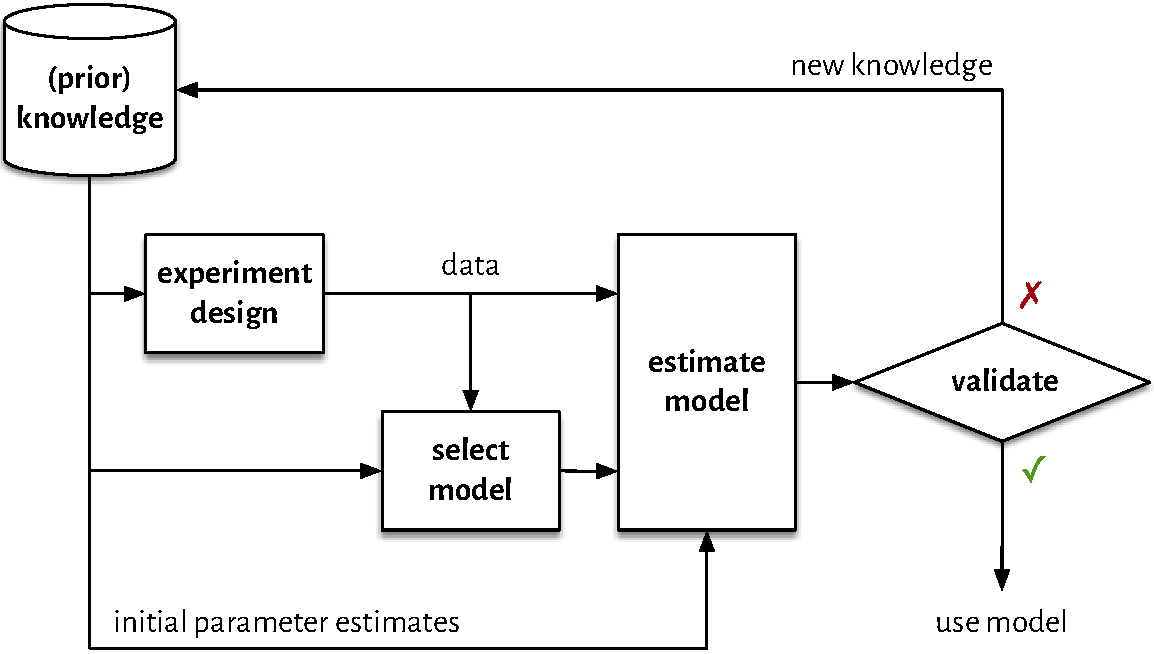
\includegraphics[width=0.9\columnwidth]{\thisDir/figs/id-cycle.pdf}
  \caption[System identification loop]{System identification loop. \disclaimer{Adapted from \citep[Figure 1.10]{Ljung1999} and \citep{Mehra1981}.}}
  \label{fig:intro:identification-cycle}
\end{figure}

\paragraph{Experiment design}
In the first step, an experiment is constructed to gain insight into the behavior of a system.
For system identification, experiment design is a question of designing input signals that will be applied to the system under test.
Typically, the design consists of constructing a signal such that the obtained model  has a small uncertainty in some sense~\citep{Goodwin1977,Mehra1974,Goodwin2006GBO,Levadi1966}.
On the one hand, if one has very precise prior information, one could even construct optimal signals~\citep{Gagliardi1967,Karlin1966,Gevers2011ExpDesign,Zarrop1979}.
Typically, the design is very sensitive to the prior knowledge of the system.
This is necessary to focus all the energy in the signal towards exciting the system dynamics as to reduce the uncertainty in the model.
However, when the prior knowledge is incomplete, uncertain or even incorrect, optimal signals can lead to very poor models as they might not excite other dynamics.
An alternative approach is to incorporate the uncertainty of the prior knowledge into the signal design.
This leads to so-called robust optimal experiment design~\citep{Rojas2012,Goodwin2006} that construct signals that optimize the worst-case model uncertainty.

The design of good experiments hence already forces the user to make a choice that can have far-reaching consequences for the model quality.

\paragraph{Select a model structure}
Once an experiment has been performed, the obtained input-output data is to be processed.
In many cases, the eventual goal of identification is to obtain a parametric model, so the user has to select a model structure and/or complexity based on both his prior knowledge and on the data.
A useful tool to help choose the model structure and/or model orders, is to inspect a nonparametric model of the system.
One such tool is the frequency response function.
For instance, by inspecting a frequency response function, a control engineer can have a rough idea of the system behavior in term of  approximate resonance frequencies, asymptotic slopes, \latin{etc.}
This gives a qualitative view of the minimally required complexity of the model and is hence a useful diagnostic tool.
However, since most parametric estimators enforce very little prior knowledge about the system, noise in the measurements can sometimes be a problem to distinguish the actual system features.

\paragraph{Estimate the model parameters}
Once the model structure has been chosen, its parameters are to be estimated.
This is done by formulating an optimization problem which serves to minimize a particular cost function.
The cost function is in essence a measure of the differences between the measured data and the model evaluated for particular parameter values.
By minimizing the cost function, the optimization procedure yields parameter values that try to minimize the misfit between the data and the model.
Unfortunately, for many identification settings, these optimization problems are non-convex~\citep{Boyd2004}.
Practically, this means that 
This means that initial values need to be available to start the optimization process.
Moreover, for poor starting values, optimization algorithms may get stuck in local minima of the cost function.
Consequently, without reasonable starting values, the `optimized' model may also be of poor quality. 


\paragraph{Validate the model}
Finally, the estimated model is validated.
Essentially, one checks whether the obtained model meets the predefined requirements, e.g. with respect to allowable uncertainty, compexity, \ldots
This can happen in a few different ways.
On the one hand, in-sample measures such as statistical tests on the value of the cost function, correlation tests on the residuals, \latin{etc.} allow to verify that the model performs well on the measured dataset.
Such approaches help to detect underfitting, where the model is not flexible enough to describe the measurements.
On the other hand, the ultimate test is to validate the model against new measurements that have not been used during the estimation.
This prevents overfitting of the model, where the model not only captures the behavior of the system but also describes the particular realization of the noise in the measurements.
The latter leads to models that are overly tuned to the measurements such that their results cannot be replicated for new measurements.
In case the model is not validated, this provides the user with new knowledge: that particular model is not good enough and at least one of the previous steps (or the prior knowledge) has to be altered.

\section{User-Friendly System Identification}
In the previous section, it has been seen that some of the system identification steps require a significant amount of prior knowledge and/or craftsmanship of the user to make good choices.

In this dissertation, we focus on developing system identification techniques that are `user-friendly'.
The availability of easy to use and fast methods has been underlined by \citet{Gevers2011Challenges}.
In this context, `user-friendly' should be understood as having a good user experience for two groups of users:
\begin{itemize}
  \item novices, without formal training in system identification, optimization, \ldots and,
  \item well-seasoned identification practitioners that are already able to build good models.
\end{itemize}
Concretely, for novice users it is important to have straightforward techniques that require little interaction.
In practice, this boils down to methods that work well for a wide class of systems.
As such, only very generic assumptions of the system under test should be made and these should be easy to interpret.

For seasoned identification practitioners, methods that require little interaction are an opportunity for automation.
This is especially important for complicated systems: systems that have high-order dynamics, \gls{MIMO} systems with a high dimensionality, and networked systems amongst others.
For such complex systems, building a model can be time-consuming and laborious if one has to supervise every step of the process.
For more advanced users, user-friendly methods can hence allow to deal with more complex systems in a shorter amount of time such that the economical cost of building a model is reduced.

In this dissertation, the focus lies on \gls{LTI} systems.
While this might seem as a very restrictive choice, this is one of the fundamental settings for system identification.
In particular, \gls{LTI} systems are a first step to build a system model.
In many cases, such a linear model is accurate enough~\citep{Schoukens2004}, e.g. to build a nominal controller, to design electrical filters and obtain a reasonable intuition of the system under test.
Also, most engineers and scientists have a good understanding of linear systems~\citep{Oppenheim1996,Mandal2007,Kailath1980} such that \gls{LTI} models align well with their prior knowledge and experience.
Nevertheless, when a linear model is not adequate, a more flexible model needs to be constructed.
Such a model could be more flexible, e.g. by relinquishing the time-invariance and/or its linearity.
However, many of those advanced modeling approaches employ \gls{LTI} models as starting values or intermediate result in building the actual non-linear~\citep{Giri2010} or time-varying model~\citep{Lataire2012,Louarroudi2014}.
As such, improvements in estimating \gls{LTI} models also indirectly improve more advanced methods.


\subsection{Contributions}
In this dissertation, we look into a few aspects of the identification workflow with the goal to make the whole process more user-friendly.
Each of these aspects will be dealt with in its own chapter.

\begin{question}[How should a good experiment be designed?]
Can we design a `good experiment' to identify a \gls{LTI} model?
Particularly, this means a robust input signal needs to be constructed without relying on extensive prior knowledge of the system.
Such a signal should cover a wide frequency band to excite all dynamics of the system during the experiment.
However, the signal should ensure that systems in different frequency bands can be identified with a specified level of accuracy.
\end{question}

\begin{question}[Which non-parametric method should be used for an \gls{FRF}?]
Developing a full parametric model for complicated systems requires considerable effort.
Instead, could we leverage non-parametric or locally parametric approaches to obtain insight in the behavior of the system?
Methods such as the \gls{LPM} and \gls{LRM} can offer good results.
However, it is not clear how these should be tuned for different circumstances (near sharp resonance peaks, in low noise circumstances, \ldots).
Can we devise simple rules that allow one to obtain good \glspl{FRF}?
\end{question}

\begin{question}[Can we estimate the peak gain of a system in a non-parametric way?]
To robustly control complicated systems, it can be overly cumbersome and even unwanted to construct high-order parametric models.
As a result, some lightly damped resonances can dominate the model uncertainty.
For robust control, this poses serious problems as such very sharp resonances are hard to observe in an \gls{FRF} measurement.
Instead, can we capture the peak gain of resonances using non-parametric models (i.e. without resorting to a global parametric model)?
\end{question}

\begin{question}[Can we avoid local minima by using smoothers?]
When a parametric model is required, this often involves solving a nonlinear optimization problem.
Such optimization problems require good initial parameter estimates to allow iterative methods to converge to a good local optimum, or, preferably even the global optimum.
Can non-parametric smoothers be used to help avoid such local optima?
\end{question}

\subsection{Outline and Publications}
   The lion's share of this thesis has been published in either peer-reviewed  journals or conferences.
   This section links my different publications to the different sections in this thesis.
   For an overview of publications grouped by type, please refer to page~\pageref{publicationList}.

\begin{refsection}
% http://tex.stackexchange.com/questions/38580/displaying-selected-bibliographic-items-in-the-body-of-the-text
% http://tex.stackexchange.com/questions/126226/how-do-i-instruct-fullcite-to-use-maxbibnames-rather-than-maxcitenames

\makeatletter
\DeclareCiteCommand{\fullcite}
  {\defcounter{maxnames}{\blx@maxbibnames}%
    \usebibmacro{prenote}}
  {\usedriver
     {\DeclareNameAlias{sortname}{default}}
     {\thefield{entrytype}}}
  {\multicitedelim}
  {\usebibmacro{postnote}}
\DeclareCiteCommand{\footfullcite}[\mkbibfootnote]
  {\defcounter{maxnames}{\blx@maxbibnames}%
    \usebibmacro{prenote}}
  {\usedriver
     {\DeclareNameAlias{sortname}{default}}
     {\thefield{entrytype}}}
  {\multicitedelim}
  {\usebibmacro{postnote}}
\makeatother

% http://tex.stackexchange.com/questions/18664/underline-my-name-in-the-bibliography
% Plus see release notes of BIBLATEX 3.3/3.4
\DeclareNameFormat{author}{%
  \nameparts{#1}%
\ifthenelse{\equal{\namepartfamily}{Geerardyn}}%
    {\textbf{\ifblank{\namepartgiven}{}{\namepartgiven\space}\namepartfamily}}%
    {\ifblank{\namepartgiven}{}{\namepartgiven\space}\ifblank{\namepartprefix}{}{\namepartprefix\space}\namepartfamily}%
\ifthenelse{\value{listcount}<\value{liststop}}%
    {\addcomma\space}
    {}}

In \chapref{sec:excitation}, quasi-logarithmic multisines are proposed as a good (robust) excitation signal. 
That chapter is based on a journal article published in \gls{IEEE} Transactions on Instrumentation \& Measurement:
\begin{itemize}
  \item \fullcite{Geerardyn2013TIM}, 
\end{itemize}
preliminary results were also presented at the 2012 \gls{IFAC} symposium on System Identification (\textsc{SYSID}) and the \gls{IEEE} International Instrumentation and Measurement Conference (\textsc{I$^{\text{2}}$MTC}):
\begin{itemize}
  \item \fullcite{Geerardyn2012IMTC}, and
  \item \fullcite{Larsson2012SYSID}.
\end{itemize}
This work has also been presented at the following local (non-refereed) conferences:
\begin{itemize}
  \item \fullcite{Geerardyn2012Benelux}, and
  \item \fullcite{Geerardyn2012ERNSI}.
\end{itemize}

The non-parametric \gls{FRF} estimation methods in \chapref{sec:nonparametric} are based on a yet-unpublished manuscript.
The so-called time-truncated \gls{LPM} that is presented in the same chapter is based on a journal published in \gls{IEEE} Transactions on Instrumentation \& Measurement:
\begin{itemize}
  \item \fullcite{Lumori2014TIM}.
\end{itemize}
In particular, this smoother enables one to reduce the effect of noise on an estimated \gls{FRF} using an automated approach.
Relatedly, a preliminary study of the \gls{LPM} in the context of lightly-damped \gls{MIMO} systems has been presented at the (non-refereed) Benelux Meeting on Systems and Control:
\begin{itemize}
    \item \fullcite{Verbeke2015Benelux}.
\end{itemize}

The use of the non-parametric \gls{FRF} estimation methods for \Hinf gain estimation (and in general the \gls{FRF} interpolation from \chapref{sec:hinf}) has been presented at the 2014 \gls{IFAC} World Conference in South Africa and the 2014 Leuven Conference on Noise and Vibration Engineering (ISMA) in Leuven:
\begin{itemize}
  \item \fullcite{Geerardyn2014IFAC},
  \item \fullcite{Geerardyn2014ISMA}.
\end{itemize}
Preliminary results have been presented at local (non-refereed) conferences:
\begin{itemize}
  \item \fullcite{Geerardyn2013Benelux},
  \item \fullcite{Geerardyn2013ERNSI},
  \item \fullcite{Geerardyn2014Benelux},
  \item \fullcite{Geerardyn2014DYSCO}, and
  \item \fullcite{Geerardyn2014ERNSI}.
\end{itemize}
Experimental work related to \chapref{sec:hinf} has also been presented at the 2015 \gls{IFAC} Symposium on System Identification (\textsc{sysid}) and :
\begin{itemize}
  \item \fullcite{Voorhoeve2015SYSID}
  \item \fullcite{Voorhoeve2015ERNSI}
\end{itemize}

The study of different initialization strategies as depicted in \chapref{sec:initvals} has been published in the \gls{IEEE} Transactions on Instrumentation \& Measurement:
\begin{itemize}
  \item \fullcite{Geerardyn2015TIM},
\end{itemize}
and also at the local (non-refereed) 2015 Benelux Meeting on Systems and Control:
\begin{itemize}
    \item \fullcite{Geerardyn2015Benelux}.
\end{itemize}

In collaboration with fellow researchers, I have written a few other publications.
However, these publications are not covered in this dissertation.

\begin{itemize}
  \item \fullcite{vanBerkel2014Automatica},
  \item \fullcite{Cooman2012SMACD},
  \item \fullcite{Cooman2012DYSCO},
  \item \fullcite{Cooman2012ERNSI}.
\end{itemize}
\end{refsection}

